\lecture{Secure Connection}{29~-~01~-~2026}
%
%
\section{Virtual Private Network}
Le VPN rappresentano una tecnologia fondamentale per estendere la sicurezza delle reti locali attraverso infrastrutture pubbliche.

Una VPN crea una connessione tra due reti locali (LAN). Sebbene fisicamente la connessione avvenga attraverso Internet, logicamente le reti sono collegate come se fossero locali.Dal punto di vista della sicurezza, il traffico viene instradato attraverso un ``tunnel di rete''  controllato dal provider della VPN.
I dati sono spesso crittografati e protetti per garantirne l'integrità. L'obiettivo principale è proteggere la privacy online e mettere in sicurezza i dati sensibili.

%
\section{Protocolli di sicurezza}
È cruciale distinguere a quale livello operano i diversi protocolli di sicurezza per comprendere come proteggono i dati.
%
\subsection{IPsec}
IPsec è un protocollo IETF progettato per aggiungere sicurezza direttamente al livello ISO/OSI 3 (livello Internet). Include un protocollo per lo scambio delle chiavi chiamato IKE (Internet Key Exchange). Si basa su due possibili intestazioni (header) con funzioni distinte:
\begin{enumerate}
    \item \textbf{AH (Authentication Header)}: Garantisce integrità, autenticazione e protezione contro attacchi di tipo replay.
    \item \textbf{ESP (Encapsulating Security Payload)}: Fornisce confidenzialità (crittografia).
\end{enumerate}

%
\subsection{SSL/TLS}
TLS (Transport Layer Security) è un protocollo IETF che aggiunge sicurezza sopra il livello 4 (transport Layer).
Vedi figura \ref{fig:tls}.
%
\paragraph{Funzionalità chiave}
\begin{itemize}
    \item Autenticazione del server (obbligatoria) e del client (opzionale);
    \item Autenticazione del messaggio e confidenzialità dei dati;
    \item Protezione contro attacchi replay.
\end{itemize}
%
\paragraph{Handshake} La comunicazione inizia con la richiesta di un servizio (es. pagina web), seguita dallo scambio di Ciphersuite, parametri di sicurezza e certificato del server. Avviene poi uno scambio di challenge/response per verificare l'identità prima di procedere allo scambio sicuro dei dati.

\begin{note}
    Le versioni di TLS precedenti alla v1.2 sono considerate obsolete.
\end{note}

\begin{figure}
    \centering
    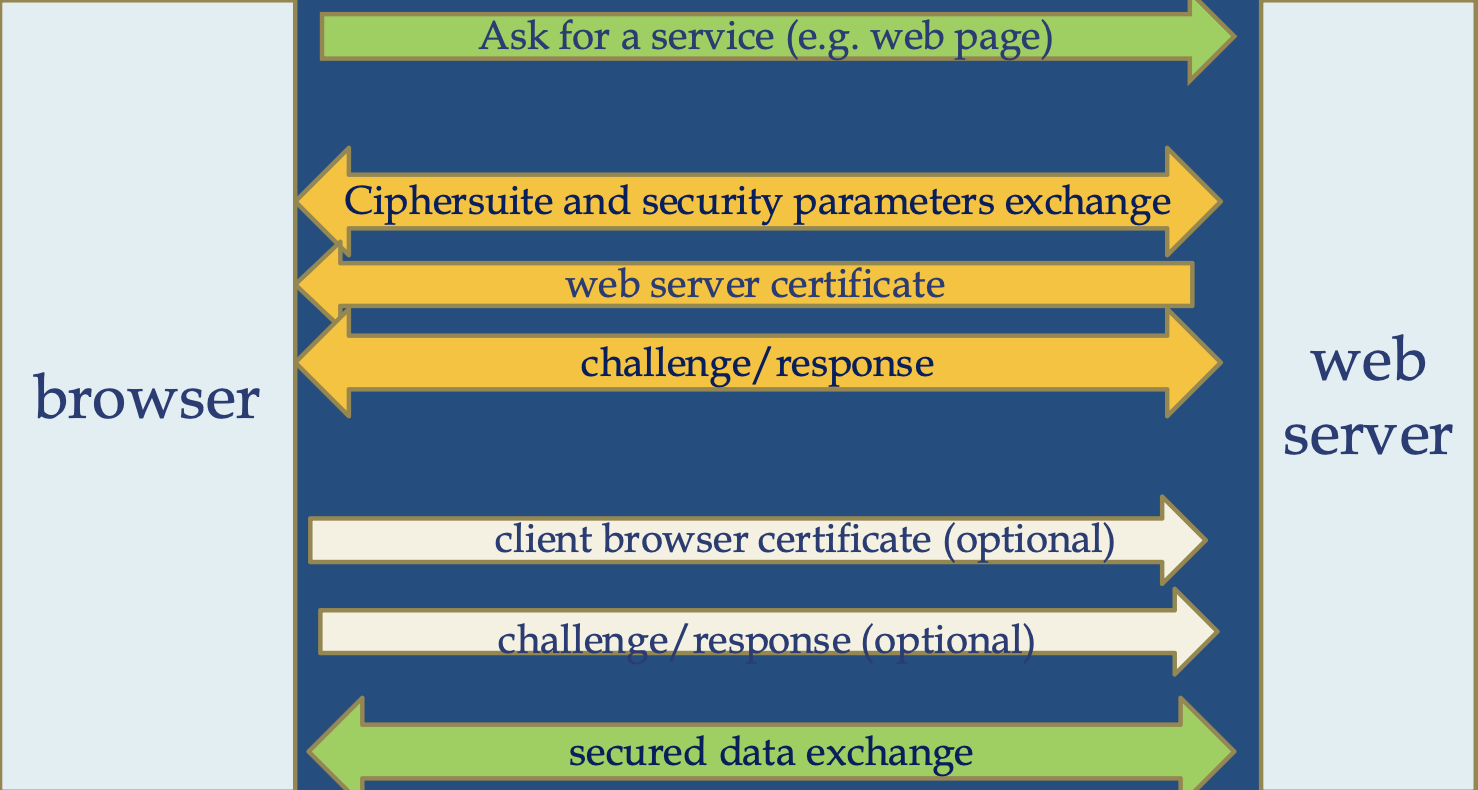
\includegraphics[width=0.7\linewidth]{assets/Screenshot 2026-01-30 at 14.29.35.png}
    \caption{TLS Exchange}\label{fig:tls}
\end{figure}

%
\subsection{SSH}
SSH (Secure Shell), specificamente nella versione 2, è un protocollo che aggiunge sicurezza al livello 4.
\begin{itemize}
    \item Offre autenticazione del server e del client;
    \item Garantisce confidenzialità e integrità dei dati;
    \item Permette il \emph{re-exchange} (nuovo scambio) delle chiavi durante la sessione.
\end{itemize}

%
\section{Network Protection}
Questa sezione si concentra sui componenti hardware e software che difendono il perimetro e l'interno della rete.
%
\subsection{Firewall}
Il firewall è un componente di sicurezza (Hardware, Software o ibrido) che monitora e controlla il traffico di rete in entrata e in uscita.
Deve essere un componente altamente sicuro e deve fungere da unico punto di contatto tra due reti.

Il suo scopo è quello di separare due reti che hanno livelli di sicurezza differenti (es. separare la Rete A/Internet a bassa sicurezza dalla Rete B ad alta sicurezza).

%
\subsection{IDS e IPS}
L'IDS (Intrusion Detection System, rilevamento) e l'IPS (Intrusion Prevention System, prevenzione) sono due sistemi di cybersecurity che servono ad identificare e a prevenire falle di sicurezza.

L'IDS (Intrusion Detection System) serve a identificare entità che utilizzano un computer o una rete in modo improprio. Utilizza due metodi principali per identificare pattern:
\begin{itemize}
    \item \textbf{Signature (Firma)}: Cerca pattern simili a comportamenti noti come ``cattivi'' (malware, attacchi noti);
    \item \textbf{Anomaly (Anomalia)}: Cerca pattern che non sono simili al comportamento ``buono'' o normale della rete.
\end{itemize}
L'IPS (Intrusion Prevention System) è l'unione di un IDS con un Firewall (in modalità dinamica e distribuita), serve a prevenire e combattere attacchi.